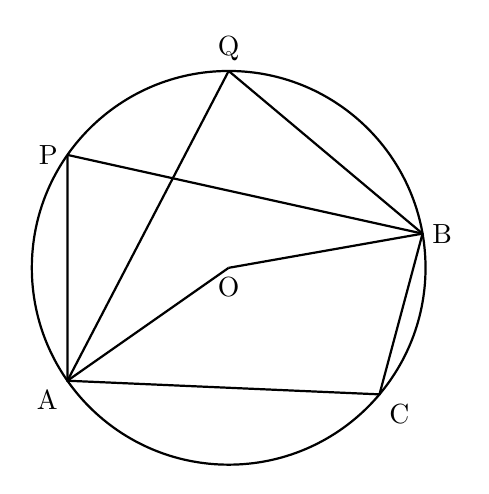
\begin{tikzpicture}[scale=1]

    % --- 1. Circle Definition ---
    % Drawing the circumscribed circle centered at O
    \coordinate (O) at (0,0);
    \draw[thick] (O) circle (2.5cm);

    % --- 2. Point Coordinates (Approximate positions based on Fig 19) ---
    % Using polar coordinates (angle:radius) to ensure they sit on the circle
    \coordinate (A) at (215:2.5);  % Bottom-left
    \coordinate (C) at (320:2.5);  % Bottom-right
    \coordinate (B) at (10:2.5);   % Middle-right
    \coordinate (Q) at (90:2.5);   % Top
    \coordinate (P) at (145:2.5);  % Top-left

    % --- 3. Drawing Lines and Segments ---
    % Outer segments (modified to erase the PQ line)
    % We draw the path from P around to Q, omitting the direct segment between them.
    \draw[thick] (P) -- (A) -- (C) -- (B) -- (Q);
    
    % Internal segments connecting vertices
    \draw[thick] (P) -- (B);      % Line PB
    \draw[thick] (Q) -- (A);      % Line QA
    
    % Central angle segments (Radii)
    \draw[thick] (O) -- (A);      % Radius OA
    \draw[thick] (O) -- (B);      % Radius OB

    % --- 4. Point Labels ---
    % Positioned exactly as they appear in the source image
    \node[below left] at (A) {A};
    \node[below right] at (C) {C};
    \node[right] at (B) {B};
    \node[above] at (Q) {Q};
    \node[left] at (P) {P};
    \node[below] at (O) {O};

\end{tikzpicture}